\chapter{Results - Vicon Test}\label{cha4}
In this chapter the algorithm from chapter \ref{cha2} is tested under different conditions. In a first part (see chapter \ref{setup}) the set up of the test is presented. In the second part (see chapter \ref{evaluation}). The different test conditions are described and the results shown.
\section{Set up}\label{setup}
To verify the performance of the Kalman filter algorithm described in chapter \ref{cha3} a ground truth is needed.  By using the motion capture system from the English company "vicon" some test were performed. The vicon system provides the position of the sensors and the orientation. Because this test has to be performed indoors no GPS signal was available. The vicon data for position added with some noise was simulated as GPS measurement and as such handed to the algorithm.The same was done with the derivative of the vicon position to provide a velocity measurement. The impact of level of noise added to the signals can be seen in chapter \ref{noise}.
The pendulum setup can be seen on the picture in figure \ref{pend_setup}. 
\begin{figure}[h]
\centering
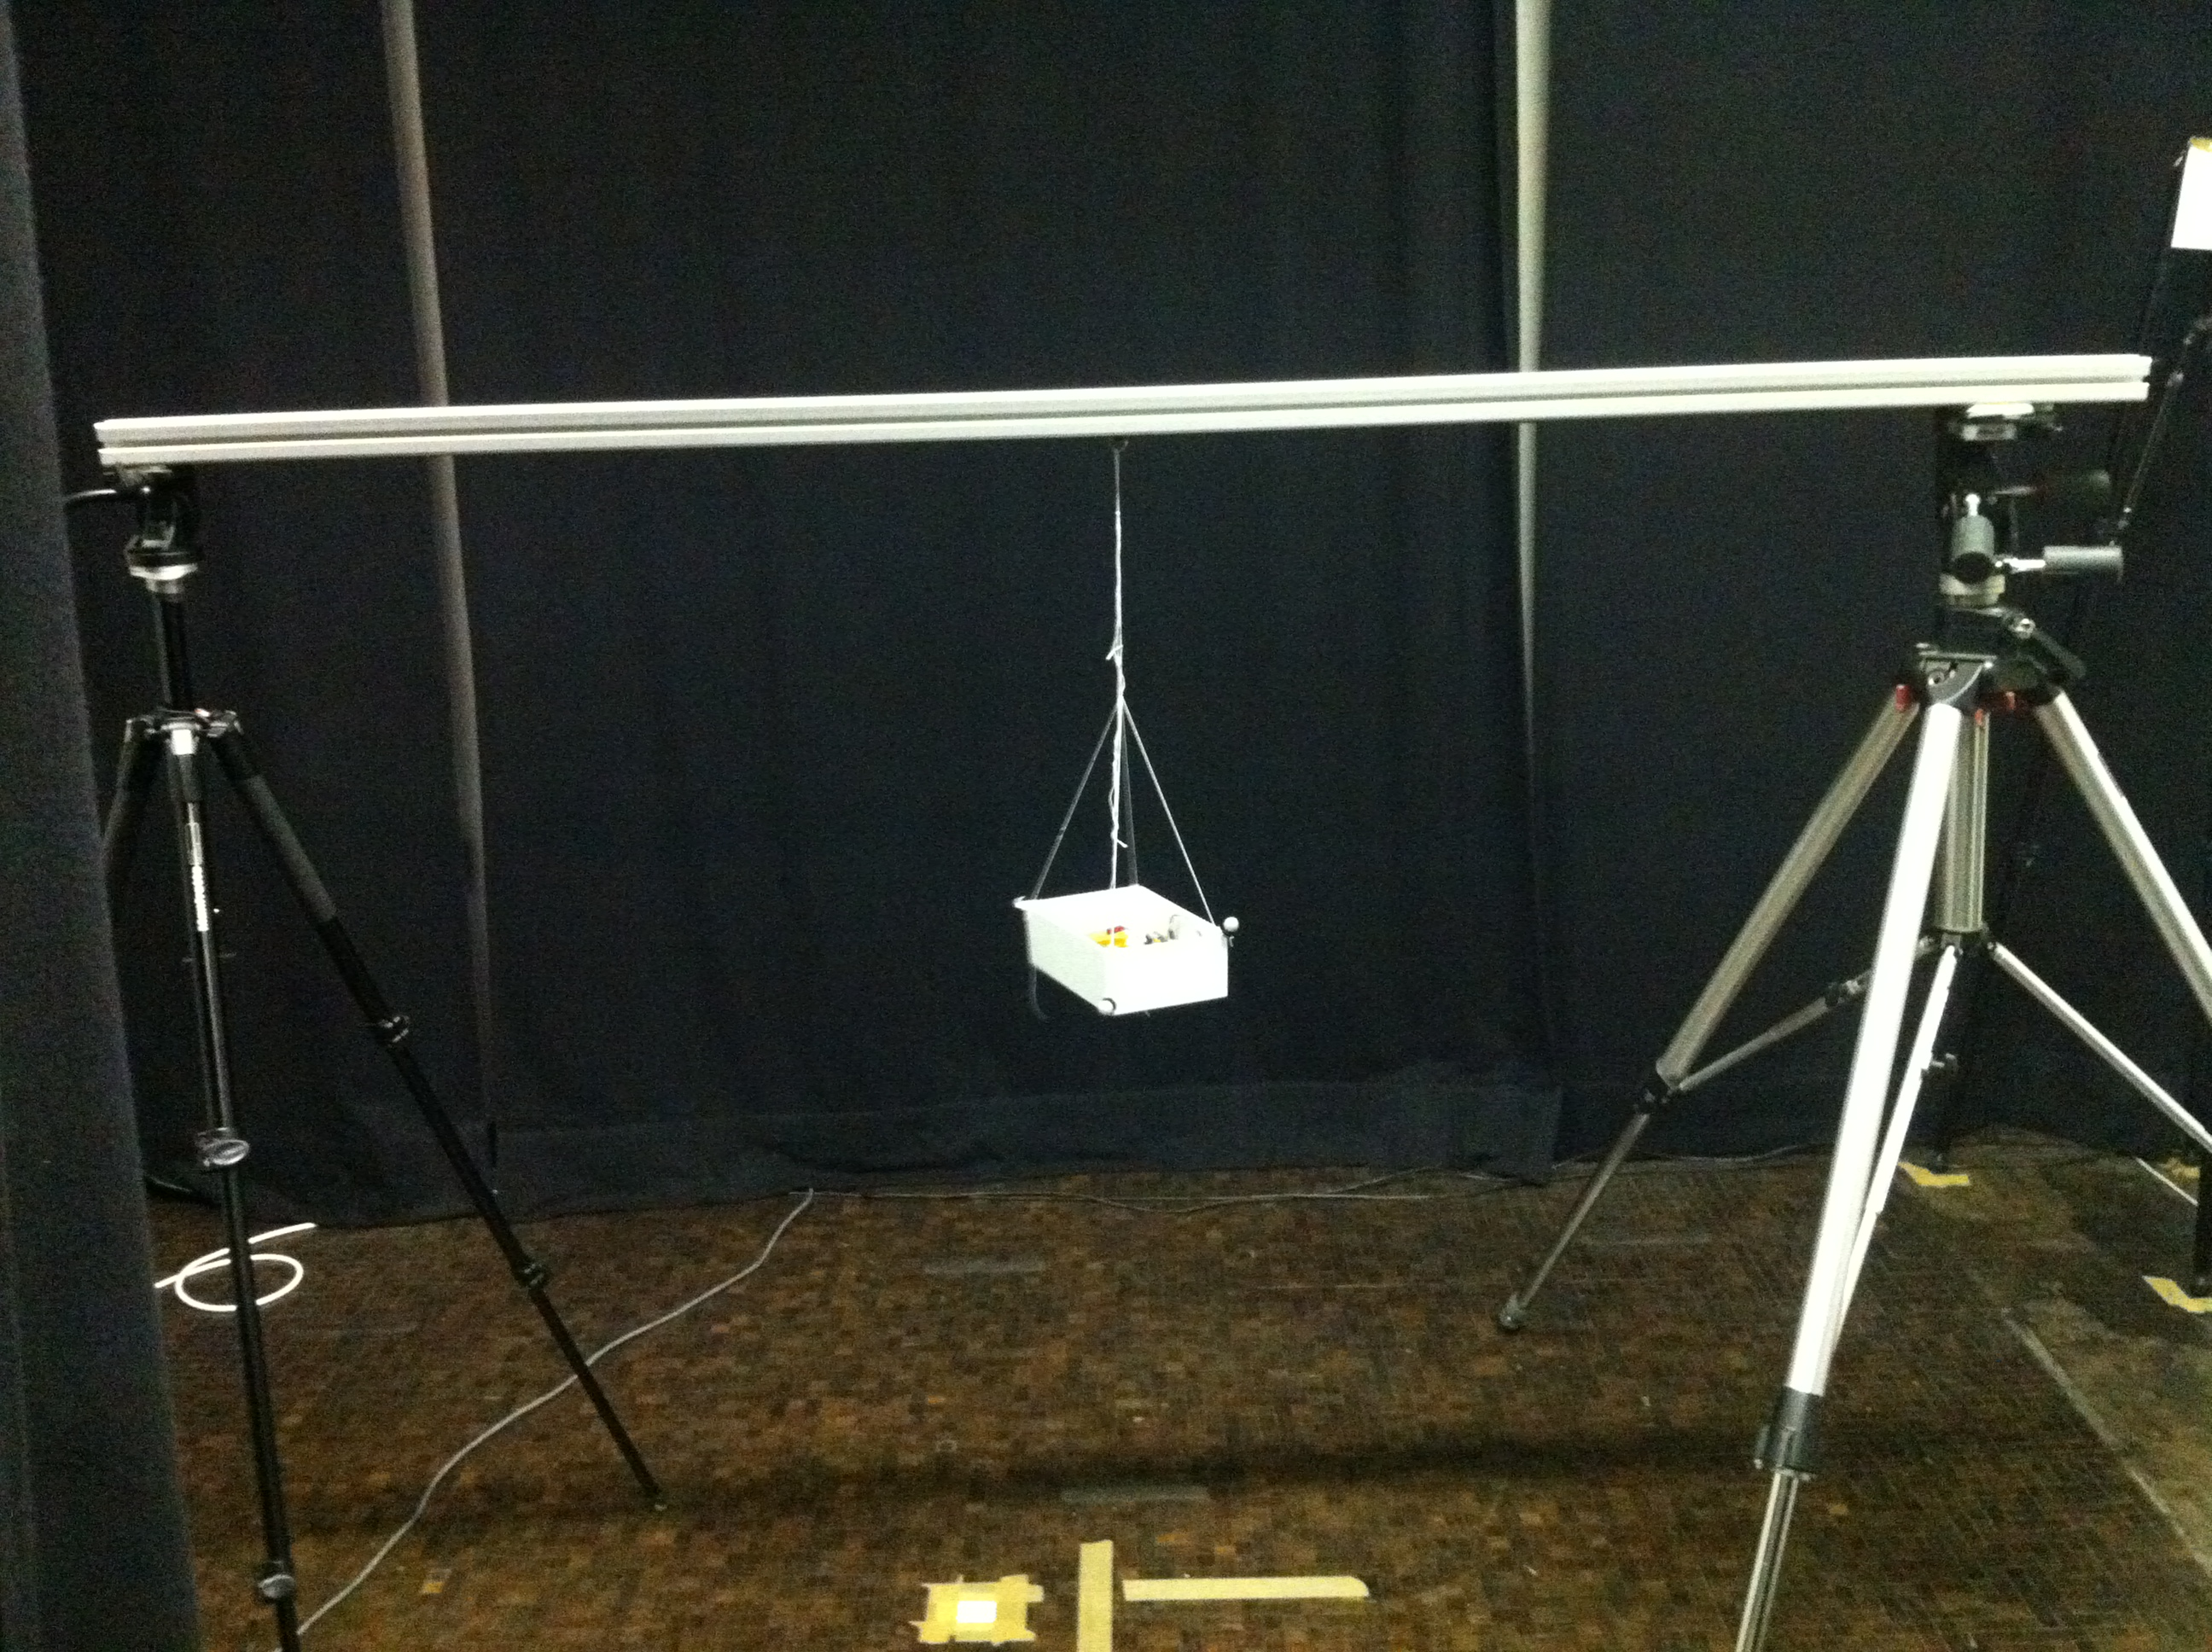
\includegraphics[width=0.8\textwidth]{vicon_bilder/IMG_0137.JPG}
\caption{Pendulum set up.}
\label{pend_setup}
\end{figure}
The box with the two sensors PX4 and MTi-G is showed in figure \ref{box_setup}.
\begin{figure}[h]
\centering
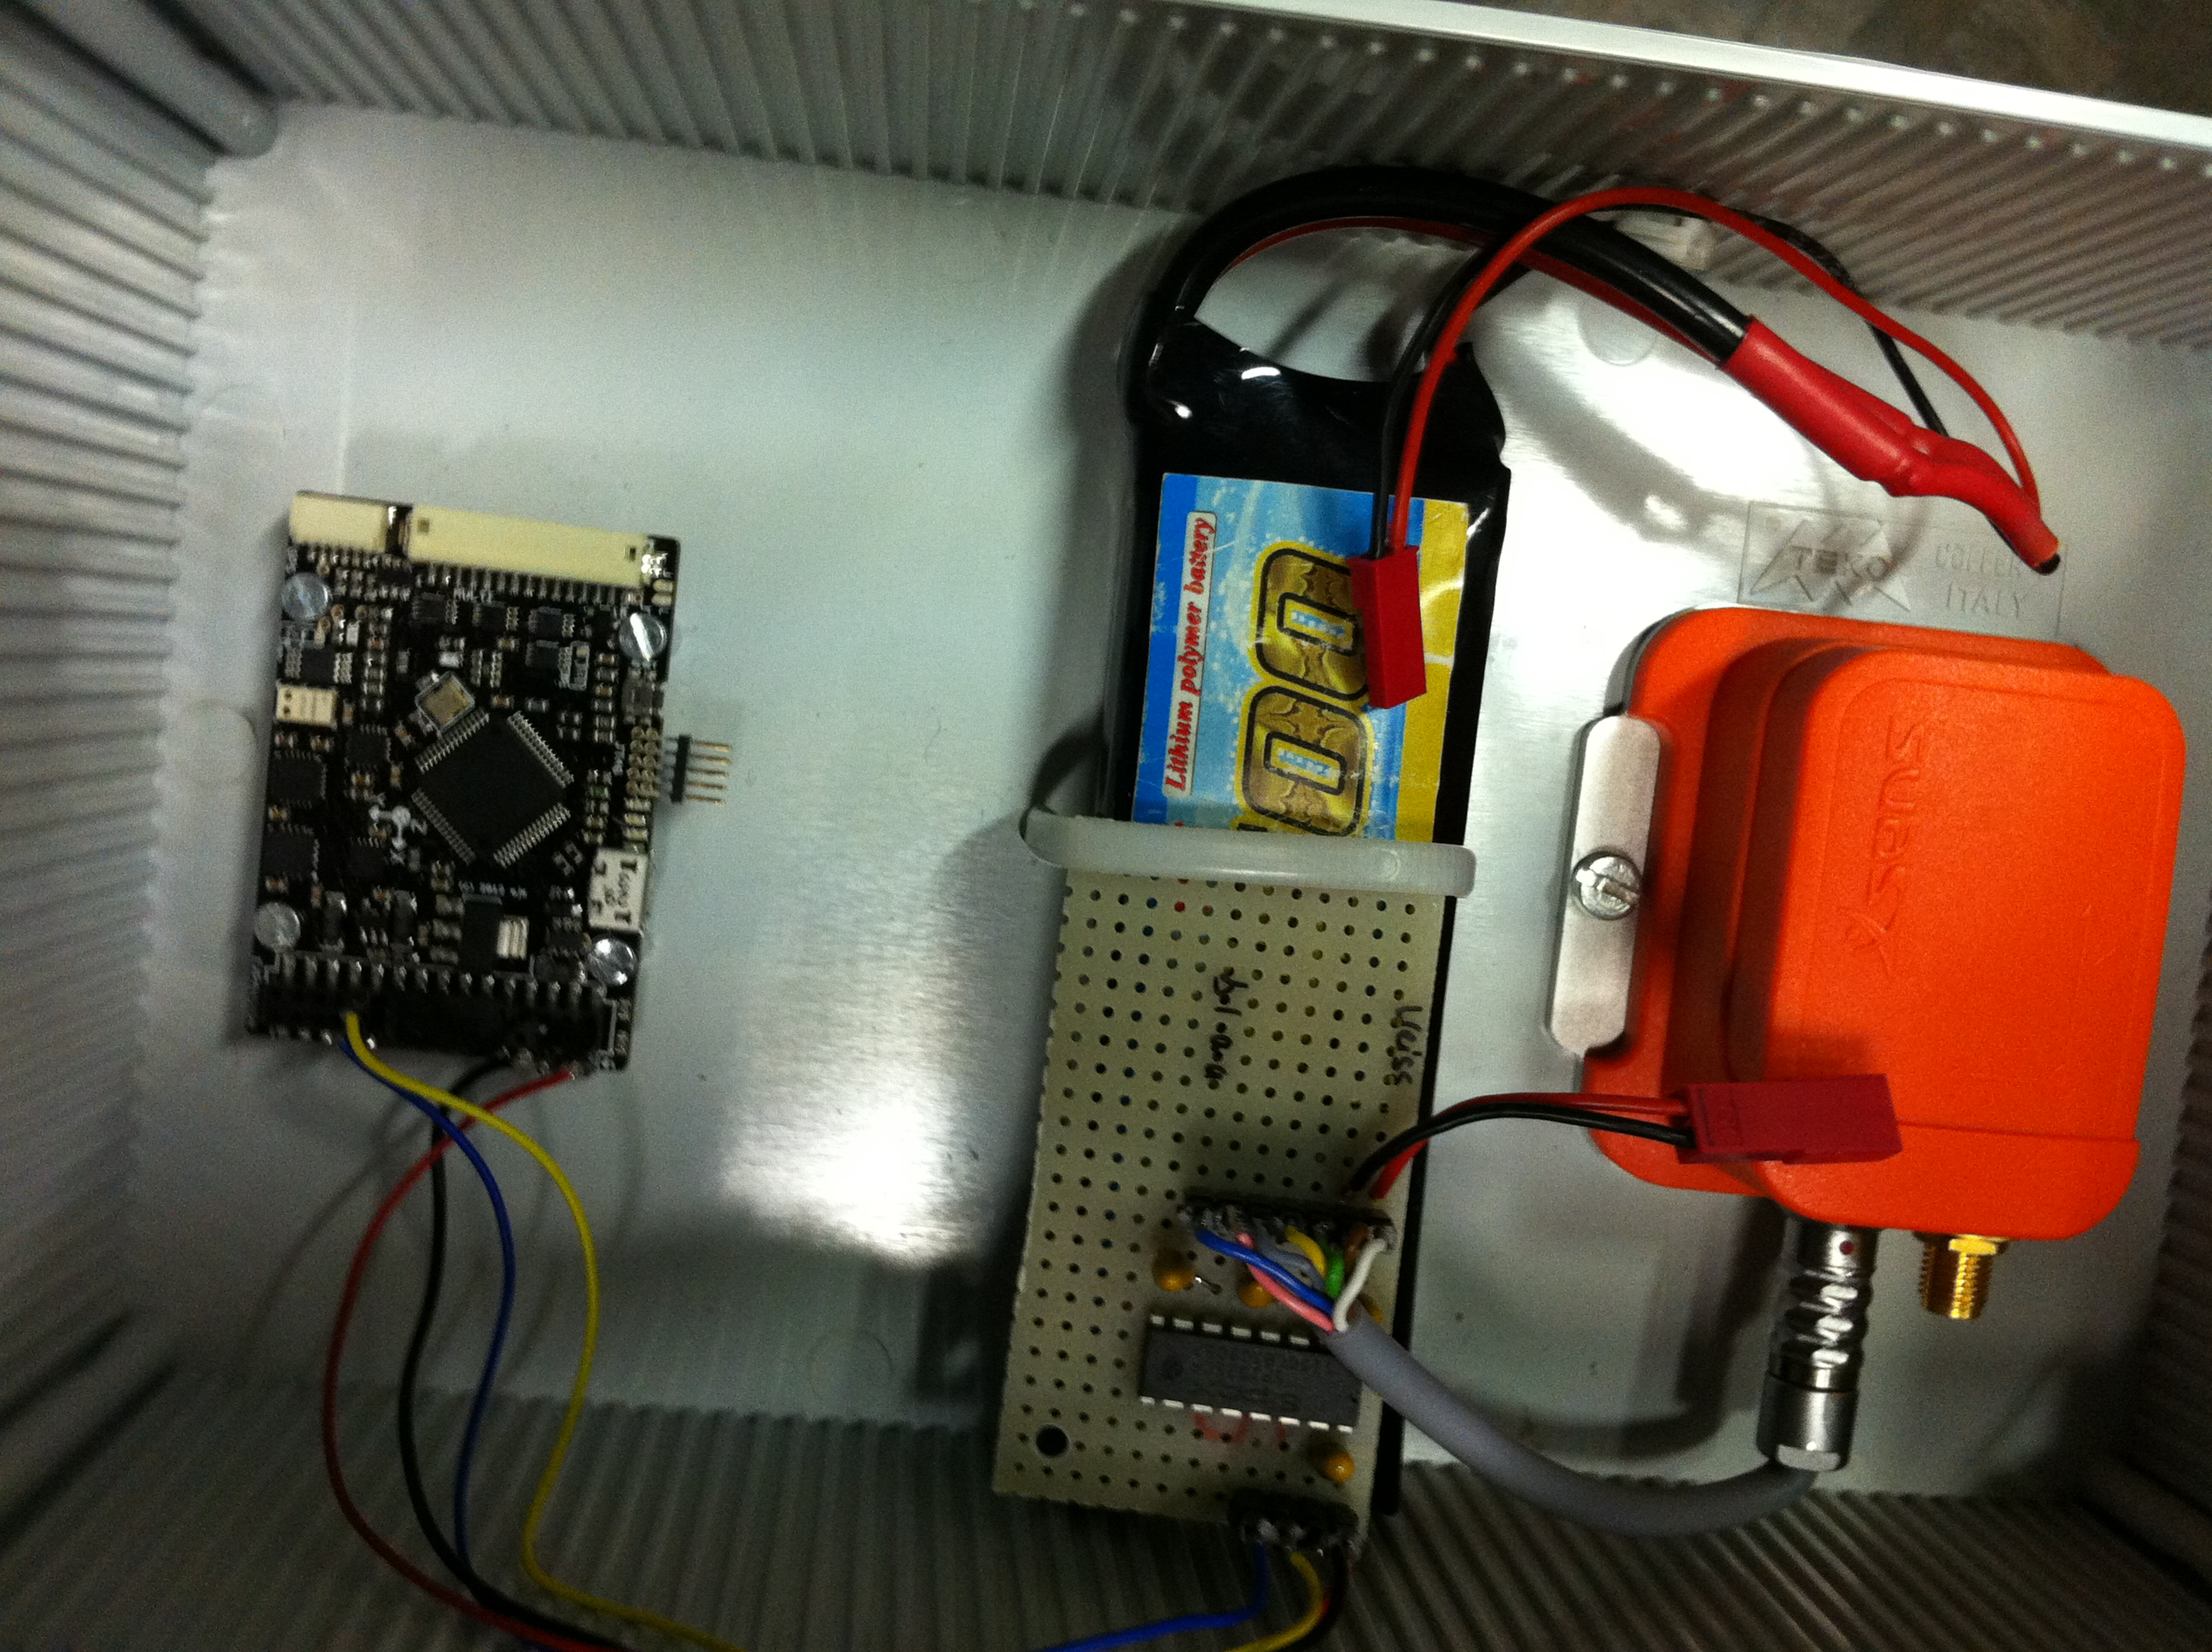
\includegraphics[width=0.8\textwidth]{vicon_bilder/IMG_0130.JPG}
\caption{Box with sensors.}
\label{box_setup}
\end{figure}
How the algorithm's state estimation differs depending on wether the measurements from the PX4 IMU or from the MTi-G IMU are used, can be read in chapter \ref{IMU_comp}.
%In addition, a Kalman Filter which does not take into account the information of a pendulum's movement has to be implemented. A free mass model state estimation is used as control algorithm. The varying results between the state estimation with using the pendulum's physical behavior and without are shown in chapter (..). SENTENCE OBSOLETE SINCE MENTIONED IN CH3???



\section{Evaluation}\label{evaluation}
Four comparisons are made to get an overview of the estimators performance. This chapter shows how different test conditions influence the performance. First it has to be verified if an estimator using a model of the pendulum's physical behavior is more accurate than a conventional Extended Kalman Filter using the free mass model as estimation model. The results of this comparison can be seen in section \ref{fmm}. In chapter \ref{noise} the estimator is tested once with a low noise GPS signal and a second time with a higher noise GPS signal. Since a GPS signal is not always available or has at least a lower frequency than the IMU measurements, the behavior of the estimator in between two GPS fixes is a main performance criteona for an estimator. In chapter \ref{no_GPS} this condition is tested. How the estimator performes with the measurements of the two IMUs is shown in section \ref{IMU_comp}. The following test are all using the MTi-G IMU except the last one in chapter \ref{IMU_comp}.

\FloatBarrier

\subsection{"Pendulum"-estimator vs. "free mass model"-estimator}\label{fmm}
In order to investigate the performance difference of the two different estimators, they were both tested with the same inputs and their respective outputs were compared. In both cases a GPS signal with a signal to noise ratio (SNR) of $-5 dB$ was used. SNR is the ratio between the desired signal and the background noise. It behaves like the smaller the ratio the higher the noise. The results are shown in Figures \ref{pos}, \ref{orientation}, \ref{pos_fmm} and \ref{orientation_fmm}. The estimator output is plotted together with the ground truth obtained from the Vicon system.
\begin{figure}[H]
\begin{center}
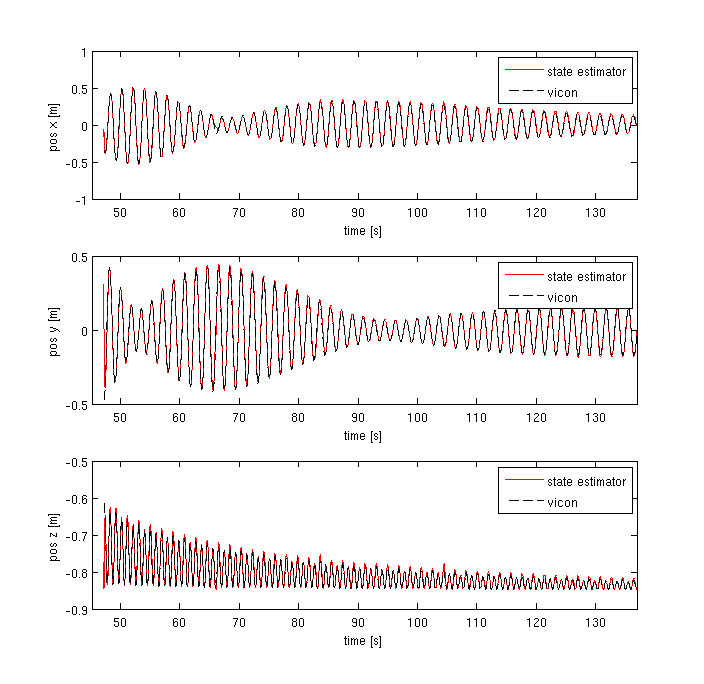
\includegraphics[width=1\textwidth]{pictures/2_2_SNR5_pos_GPS.png}
\caption{Estimation of the position using the "Pendulum"-estimator compared to the ground truth obtained from the Vicon system.}
\label{pos}
\end{center}
\end{figure}
\begin{figure}
\centering
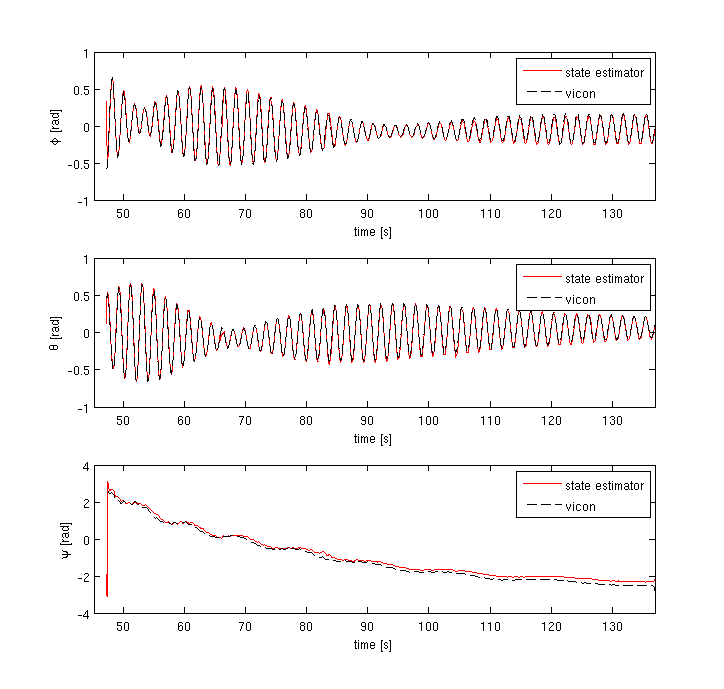
\includegraphics[width=1\textwidth]{pictures/2_2_SNR5_orientation_GPS.png}
\caption{Estimation of the orientation using the "Pendulum"-estimator compared to the ground truth obtained from the Vicon system.}
\label{orientation}
\end{figure}
\begin{figure}[hb]
\centering
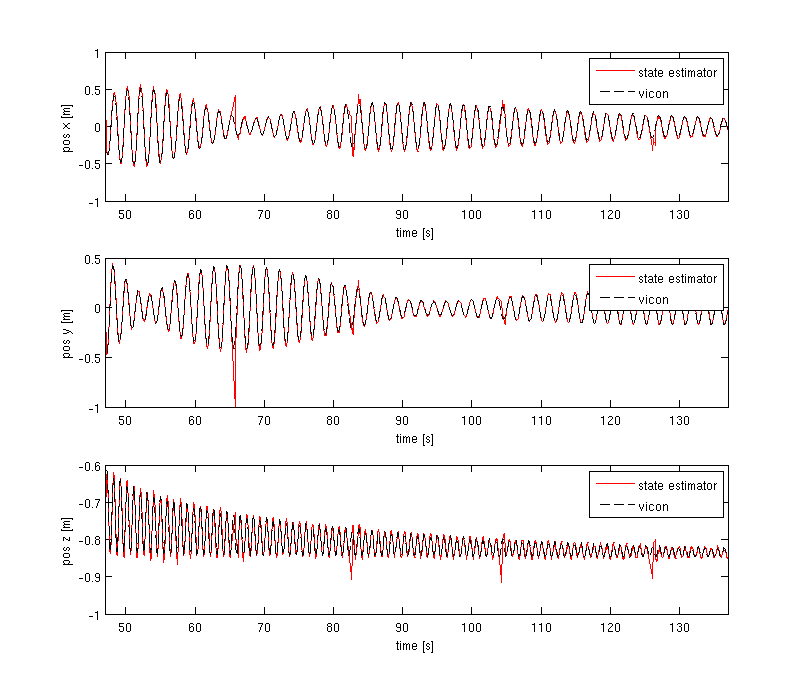
\includegraphics[width=1\textwidth]{pictures/2_2_fmm_SNR5_pos_GPS.png}
\caption{Estimation of the position using the "free mass model"-estimator compared to the ground truth obtained from the Vicon system.}
\label{pos_fmm}
\end{figure}
\begin{figure}[hb]
\centering
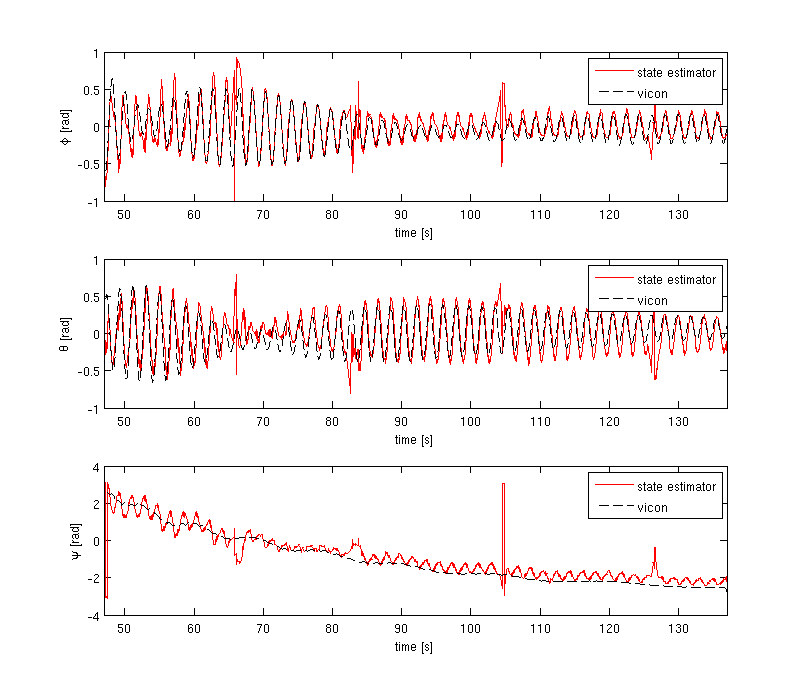
\includegraphics[width=1\textwidth]{pictures/2_2_fmm_SNR5_orientation_GPS.png}
\caption{Estimation of the orientation using the "free mass model"-estimator compared to the ground truth obtained from the Vicon system.}
\label{orientation_fmm}
\end{figure}

From these plots it can be seen, that the accuracy of the position estimation is not very much dependent of the estimator. However, due to its reduced number of degrees of freedom, the "Pendulum"-estimator clearly outperforms the "free mass model"-estimator in the accuracy of the orientation. 
To quantify these observations, the errors in position and orientation are calculated. The position error is calculated by the norm of the difference between estimated position and the effective position: 
\begin{equation}
error= \left| \begin{bmatrix} vicon_{pos\;x} \\ vicon_{pos\;y} \\ vicon_{pos\;z} \end{bmatrix}-\begin{bmatrix}state_{pos\;x} \\ state_{pos\;y} \\ state_{pos\;z}  \end{bmatrix}\right|
\end{equation}
For the orientation only the error of the $\Psi$ angle is calculated since the errors in the other two angles are represented by the error in position. 
The plots of these errors can be seen in Figures \ref{error_5snr} and \ref{error_5snr_fmm}. 
\begin{figure}[hb]
\centering
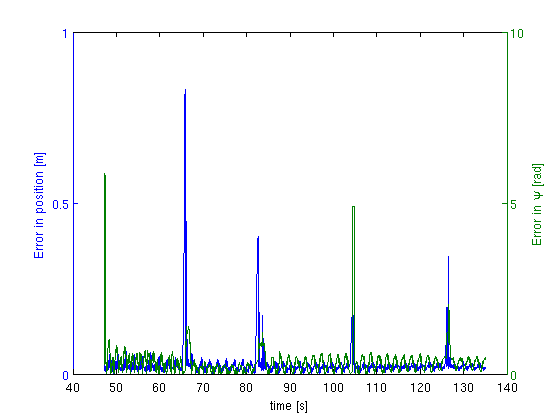
\includegraphics[width=1\textwidth]{pictures/2_2_fmm_SNR5_errors_GPS.png}
\caption{Error in position and orientation for the "free mass model"-estimator.}
\label{error_5snr_fmm}
\end{figure}
When calculating the mean value of the error, starting at the time, when the estimator is settled down, the following results are obtained:
\begin{eqnarray}
meanError_{pos}^{pendulum}&=&0.0162\;m \\ meanError_{pos}^{fmm}&=&0.0280\;m \\ meanError_{\Psi}^{pendulum}&=& 0.1440\;rad\\ meanError_{\Psi}^{fmm}&=& 0.3227 \;rad
\end{eqnarray} 

\FloatBarrier

\subsection{Noise of the GPS}\label{noise}
The quality of the received GPS signal can vary according to the GPS unit used or due to different circumstances. The weather conditions or  an acceleration as we have seen in chapter \ref{cha2} can have an influence on the signals quality. As mentioned before is the GPS signal in the vicon test only simulated according the vicon data. This has the advantage of being able to use a GPS with different SNR since this is artificially added on the vicon's position data.
\begin{figure}[hb]
\centering
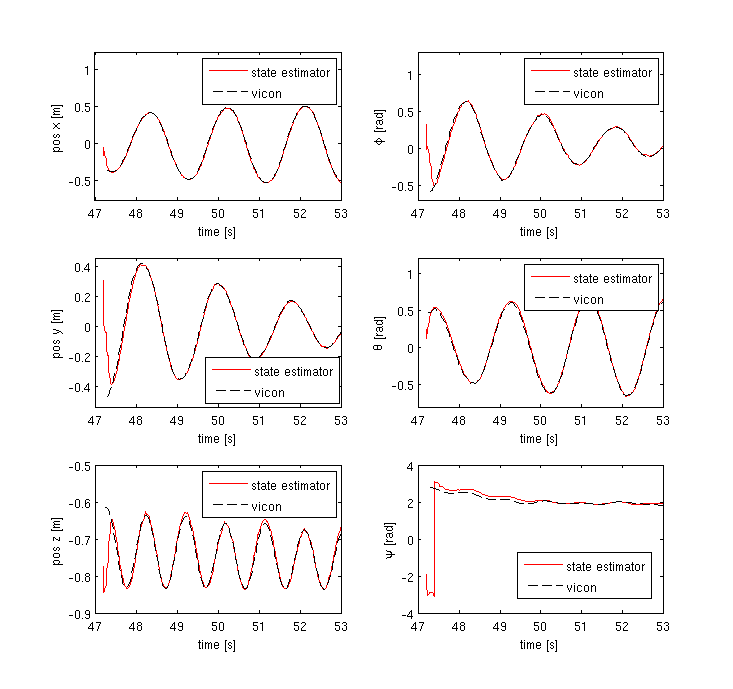
\includegraphics[width=1\textwidth]{pictures/2_2_SNR5_detail_GPS.png}
\caption{GPS signal with a SNR of -5 dB.}
\label{detail_5snr}
\end{figure}
\begin{figure}[hb]
\centering
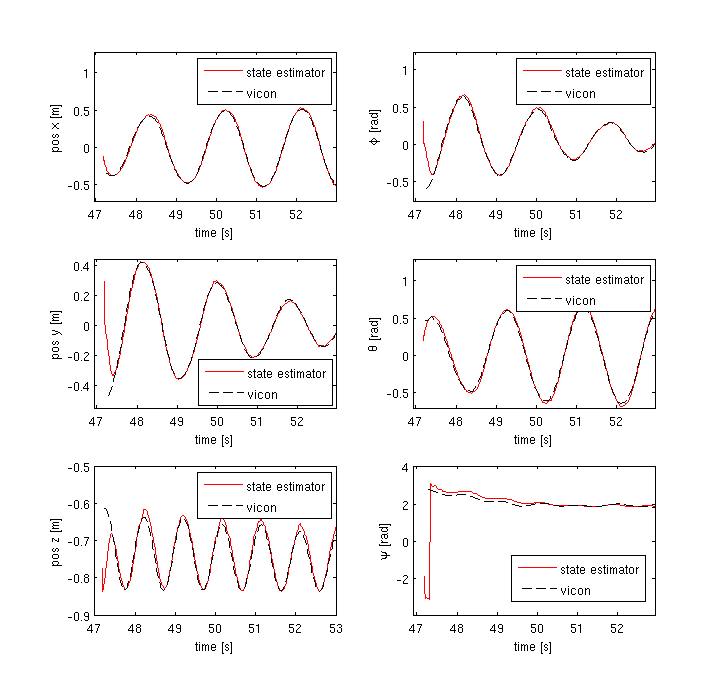
\includegraphics[width=1\textwidth]{pictures/2_2_SNR25_detail_GPS.png}
\caption{GPS signal with a SNR of -25 dB.}
\label{detail_25snr}
\end{figure}
The estimator output somehow differs, but the noise level does not have a strong impact. In the algorithm, the noise covariance matrixes are adjusted depending on the input signal's SNR. In the first case of a $-5\; dB$ SNR the variance of the GPS position and velocity are defined as $0.001 m$ and $0.01 m/s$ respectively. In the second case with a SNR of $-25\; dB$ the variance in the algorithm is increased to $0.01 m$ for the position and $0.05 m/s$ for the velocity.
In figure \ref{error_5snr} and figure \ref{error_25snr} the errors in position and orientation are plotted for the $-5\; dB$ and $-25\; dB$ GPS signals respectively. 
\begin{figure}[hb]
\centering
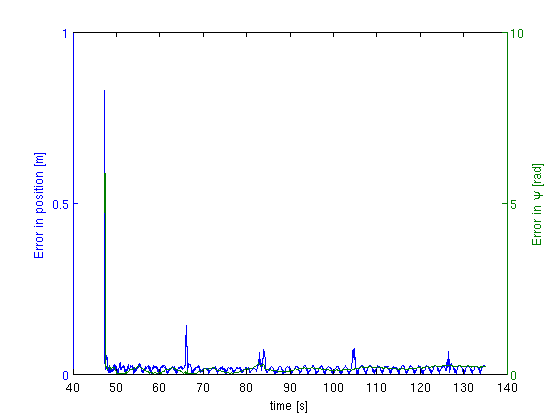
\includegraphics[width=1\textwidth]{pictures/2_2_SNR5_errors_GPS.png}
\caption{Error in position and orientation using a GPS signal with a SNR of -5 dB.}
\label{error_5snr}
\end{figure}
\begin{figure}[hb]
\centering
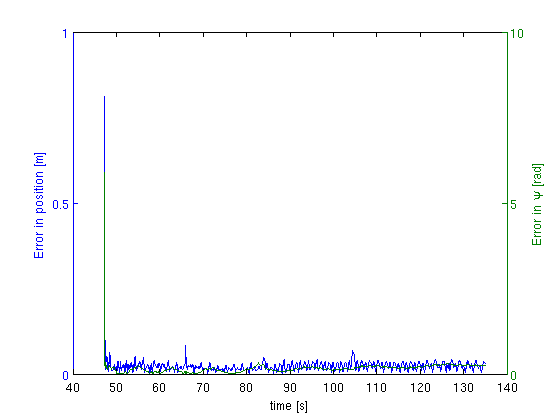
\includegraphics[width=1\textwidth]{pictures/2_2_SNR25_errors_GPS.png}
\caption{Error in position and orientation 	using a GPS signal with a SNR of -25 dB.}
\label{error_25snr}
\end{figure}
%The error is calculated by the norm of the difference between estimated position and the effective position: 
%\begin{equation}
%error= \left\vert \begin{bmatrix} vicon_{pos\;x} \\ vicon_{pos\;y} \\ vicon_{pos\;z} \end{bmatrix}-\begin{bmatrix}state_{pos\;x} \\ state_{pos\;y} \\ state_{pos\;z}\right\vert \end{bmatrix}
%\end{equation}
For the orientation only the error of the $\Psi$ angle is calculated since the errors in the other two angles are represented by the error in position. When calculating the mean value of the error, starting at the point, when the estimator is settled down, the following results are obtained:
\begin{eqnarray}
meanError_{pos}^{-5\;dB}&=&0.0162\;m \\ meanError_{pos}^{-25\;dB}&=&0.0223\;m \\ meanError_{\Psi}^{-5\;dB}&=& 0.1440\;rad\\ meanError_{\Psi}^{-25\;dB}&=& 0.1584 \;rad
\end{eqnarray}
And a ratio of:
\begin{eqnarray}
\frac{meanError_{pos}^{-5\;dB}}{meanError_{pos}^{-25\;dB}}&=&0.7265 \\ \frac{meanError_{\Theta}^{-5\;dB}}{meanError_{\Theta}^{-25\;dB}}&=&0.9091
\end{eqnarray}

\FloatBarrier

\subsection{GPS outage}\label{no_GPS}
As explained earlier in this chapter, the performance of a estimator without having a GPS signal is an important criterion. For this purpose, the algorithm was run without any position or velocity measurements in the input. In figure \ref{detail:_noGPS} a detail of the plot is shown.
\begin{figure}[hb]
\centering
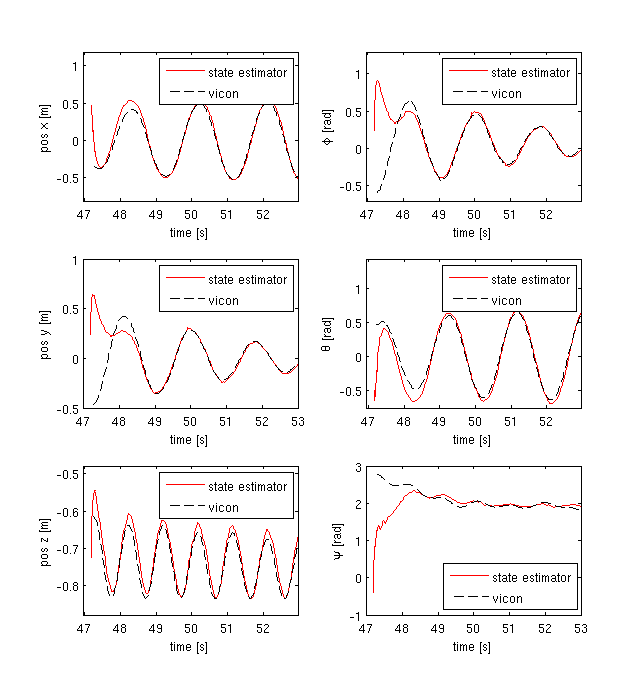
\includegraphics[width=1\textwidth]{pictures/2_2_detail_noGPS.png}
\caption{Estimation of the states without GPS signal.}
\label{detail_noGPS}
\end{figure}
As can be seen, the estimator is able to very accurately estimate the state of the system only using the IMU measurements. In this case the MTi-G data was used. Again can the error of the estimated position compared to the true position, as well as the difference between the estimated angle of $\Psi$ and the true angle can be calculated and plotted. This is done in Figure \ref{error_noGPS}. The mean value of this error is calculated in the same way as the error between the different noise levels in chapter \ref{noise}.
\begin{figure}[hb]
\centering
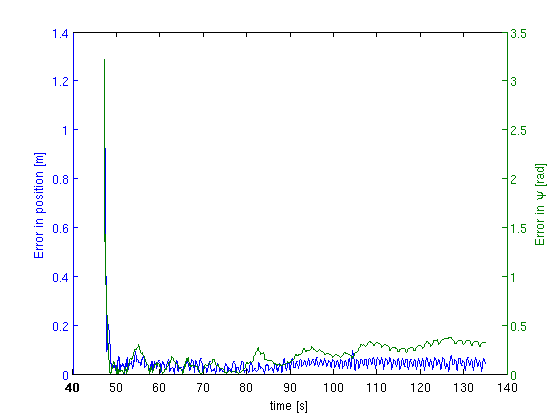
\includegraphics[width=1\textwidth]{pictures/2_2_errors_noGPS.png}
\caption{Error in position and orientation only using IMU measurements and no GPS data.}
\label{error_noGPS}
\end{figure}
The fact that no GPS data is available has an influence on the time it takes the estimator to settle. Without the accurate GPS signal, it takes between one and two seconds while the accurate information on position and velocity drag the estimator to its correct state in a few tenths of a second. Furthermore, the overall error levels are slightly higher without the GPS data ($0.0393 m$ compared to $0.0162 m$ for the position and $0.1947 rad$ compared to $0.144 rad$ for $\Psi$). 

This behaviour is also the big advantage of the pendulum model compared to the free mass model. While the first does not dramatically change its performance, the latter is very much dependent on a GPS signal. The "free mass model"-estimator was used on a GPS signal that contained a simulated GPS outage from $t=75 s$ to $t=78 s$. During that time, the position and orientation both drift away from the true values. However, upon reaquiring a GPS fix, the estimator returns very fast to its correct state, as can be seen in Figure \ref{detail_fmm_outage}.

\begin{figure}[hb]
\centering
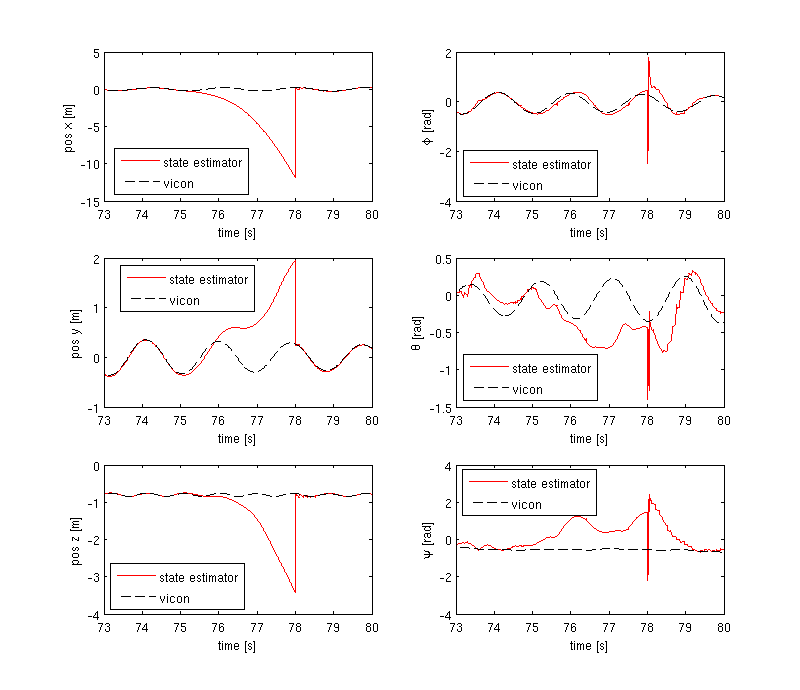
\includegraphics[width=1\textwidth]{pictures/2_2_fmm_SNR5_detail_GPSoutage.png}
\caption{"Free mass model" estimator during a GPS outage from $t=75 s$ to $t=78 s$.}
\label{detail_fmm_outage}
\end{figure}

\FloatBarrier
\subsection{The MTi-G unit versus the PX4 unit}\label{IMU_comp}
In this section the influence of the different IMU's on the estimator is presented. The above test of the estimator without having a GPS signal is carried out again.But this time using the PX4 IMU data instead of the MTi-G data. %In figure \ref{detail_no_GPS_P} the same detail is shown. 
%\begin{figure}[hb]
%\centering
%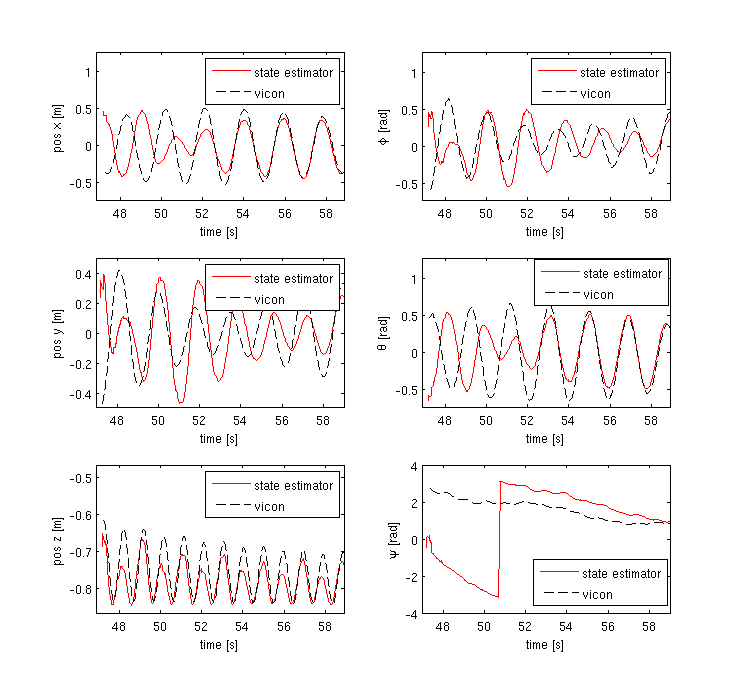
\includegraphics[width=1\textwidth]{pictures/2_2_P_detail_noGPS.png}
%\caption{Estimation of the states without GPS and the help of the PX4 IMU.}
%\label{detail_noGPS_P}
%\end{figure}
Quite surprisingly, the performance of the estimator degrades significantly compared to the MTi-G. The algorithm takes a lot longer to settle (between five and ten seconds) and the overall error is higher ($0.0743 m$ compared to $0.0393 m$ for the position and $0.241 rad$ compared to $0.1947 rad$ for $\Psi$). The plot of the errors can be found in figure \ref{error_noGPS_P}. 
\begin{figure}[h]
\centering
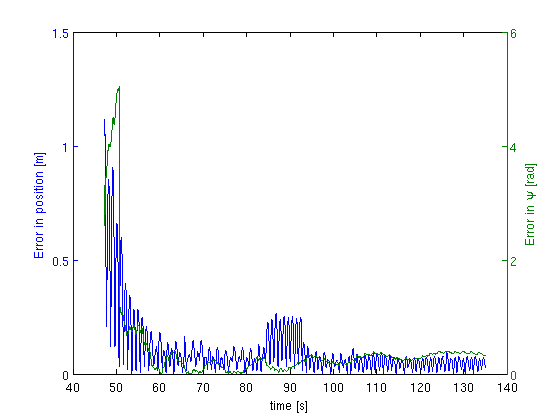
\includegraphics[width=1\textwidth]{pictures/2_2_P_errors_noGPS.png}
\caption{Error of the estimation of the states without GPS using only the PX4 IMU.}
\label{error_noGPS_P}
\end{figure}
In figure all mean errors are summarized.
\begin{figure}[hb]
\centering
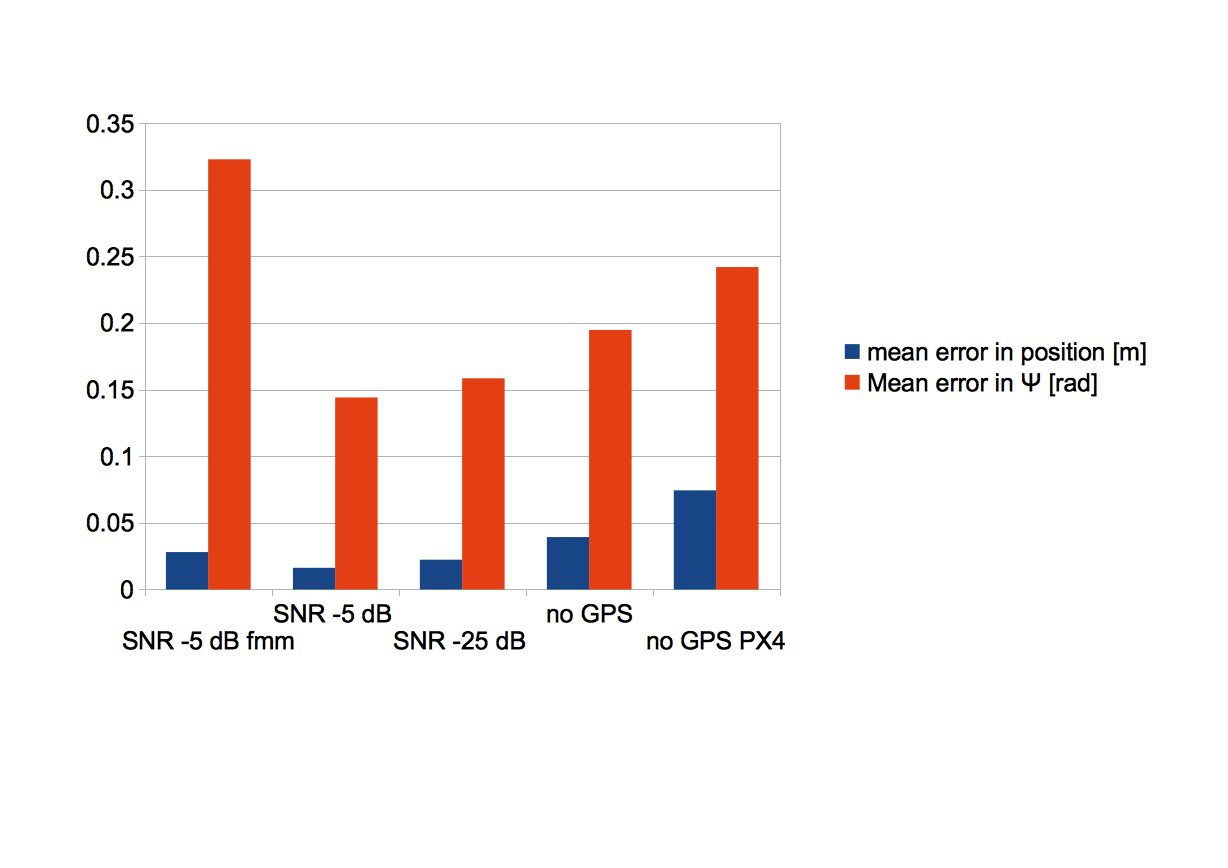
\includegraphics[width=1\textwidth]{pictures/mean_error.png}
\caption{All mean errors. Where fmm stands for free mass model which is used only in the first error calculation. All errors were calculated using the MTi-G IMU. Only the last one is using the PX4 Unit.}
\label{mean_error}
\end{figure}

%\begin{table}[h]
%\centering
%\begin{tabular}{|c|c|c|c|c|}
% \hline
% Ratios &  meanError_{pos}^{5\;dB} & meanError_{pos}^{25\;dB} & meanError_{pos}^{no GPS\;MTi-G} & meanError_{pos}^{no GPS\;PX4} \\
% \hline
% meanError_{pos}^{5\;dB} & $ 1$ && &     \\
% \hline
% meanError_{pos}^{25\;dB} & & $1$ & &  \\
% \hline
% meanError_{pos}^{no GPS\;MTi-G} &  & & 1 &   \\
%\hline
%meanError_{pos}^{no GPS\;PX4} & & & & 1\\
%\hline
%\end {tabular}
%\caption{ratio pos.}
%\label{ratio_pos}
%\end{table}



